\clearpage
\makeatletter
\efloat@restorefloats
\makeatother


\begin{appendix}
\section{}
\hypertarget{fit-to-data}{%
\subsection{Fit to data}\label{fit-to-data}}

Model fit was assessed by testing to what extent simulations obtained
from the model fit the observed data. From each model we obtained 100
simulations (predictions). These can be found in Figure
\ref{fig:prediction}. The model predictions fitted the data
substantially better for the mixture models. The worse fit was observed
for the single distribution Gaussian model which predicted large amounts
of negative keystroke intervals which are implausible. Using a
log-normal distribution removed these negative keystroke intervals.

\begin{figure}

{\centering 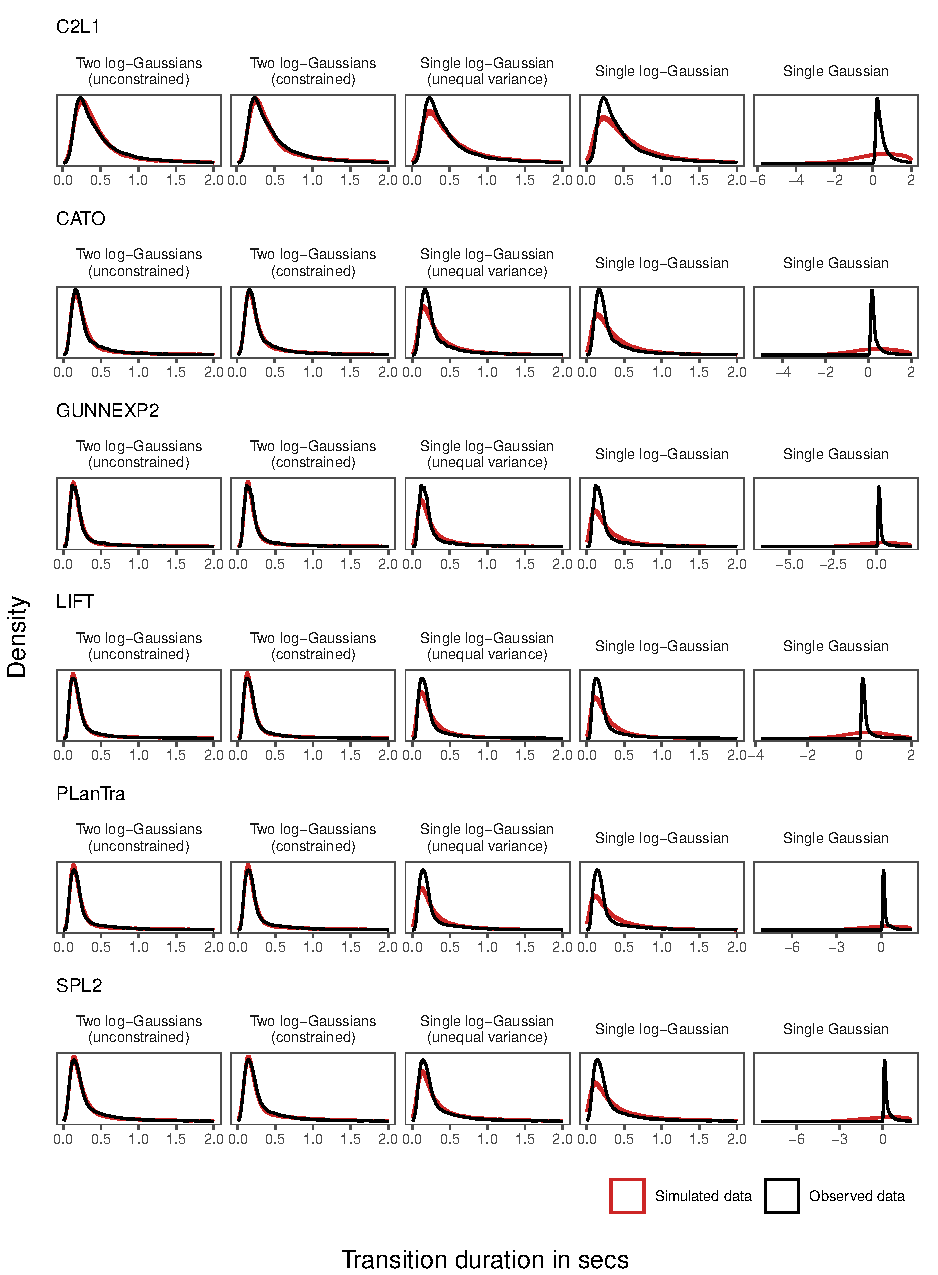
\includegraphics{figures/fitplots} 

}

\caption{Fit to data with models (distribution type) above the plots. Comparison of 50 simulations to observed data summarised by model. For illustration the x-axis was truncated at 2 secs.}(\#fig:prediction)
\end{figure}
\end{appendix}
